% !TEX root = ../main.tex
\section{Introduction}
\label{introduction}

An often-cited statistic is that data scientists spend 80\% of their time finding,
preparing, integrating, and cleaning data sets. The remaining 20\% is spent doing
the desired analytic tasks. In practice, 80\% may be a lower bound; for example
one data officer, Mark Schreiber of Merck, a large pharmaceutical company,
estimates that data scientists in Merck spend 98\% of their time on ``grunt
work'' and only one hour per week on ``useful work''.

In this paper, we present \dcv, a system we are building at MIT, QCRI, Waterloo,
and TU Berlin, whose main purpose is to decrease the ``grunt work factor'' by
helping data scientists to (i)~quickly {\it discover} data sets of interest from
large numbers of tables; (ii)~{\it link} relevant data sets; (iii)~{\it compute} answers from the
disparate data stores that host the discovered data sets; (iv)~{\it clean} the
desired data; and (v)~{\it iterate} through these tasks using a workflow
system, as data scientists often perform these tasks in different orders.


\dcv consists of two major components, as shown in Figure~\ref{fig:arch}.  The
{\it offline component} indexes and profiles data sets;  these profiles are
stored  in a linkage graph, which is used to process workflow queries online.
Data sets in \dcv consist of structured data, which may be stored in relational
databases, spreadsheets, or other structured formats. In the remainder of the
paper, we use the term {\it tables} or {\it data sets} to refer to these.  The
{\it online component} involves executing a user-supplied workflow that consists
of a mix of discovery, join path selection, and cleaning operations on data
sets, all supported via interactions with the linkage graph. We elaborate on
each module in the remainder of this section, using Merck as an example.


\begin{figure}[!t]
%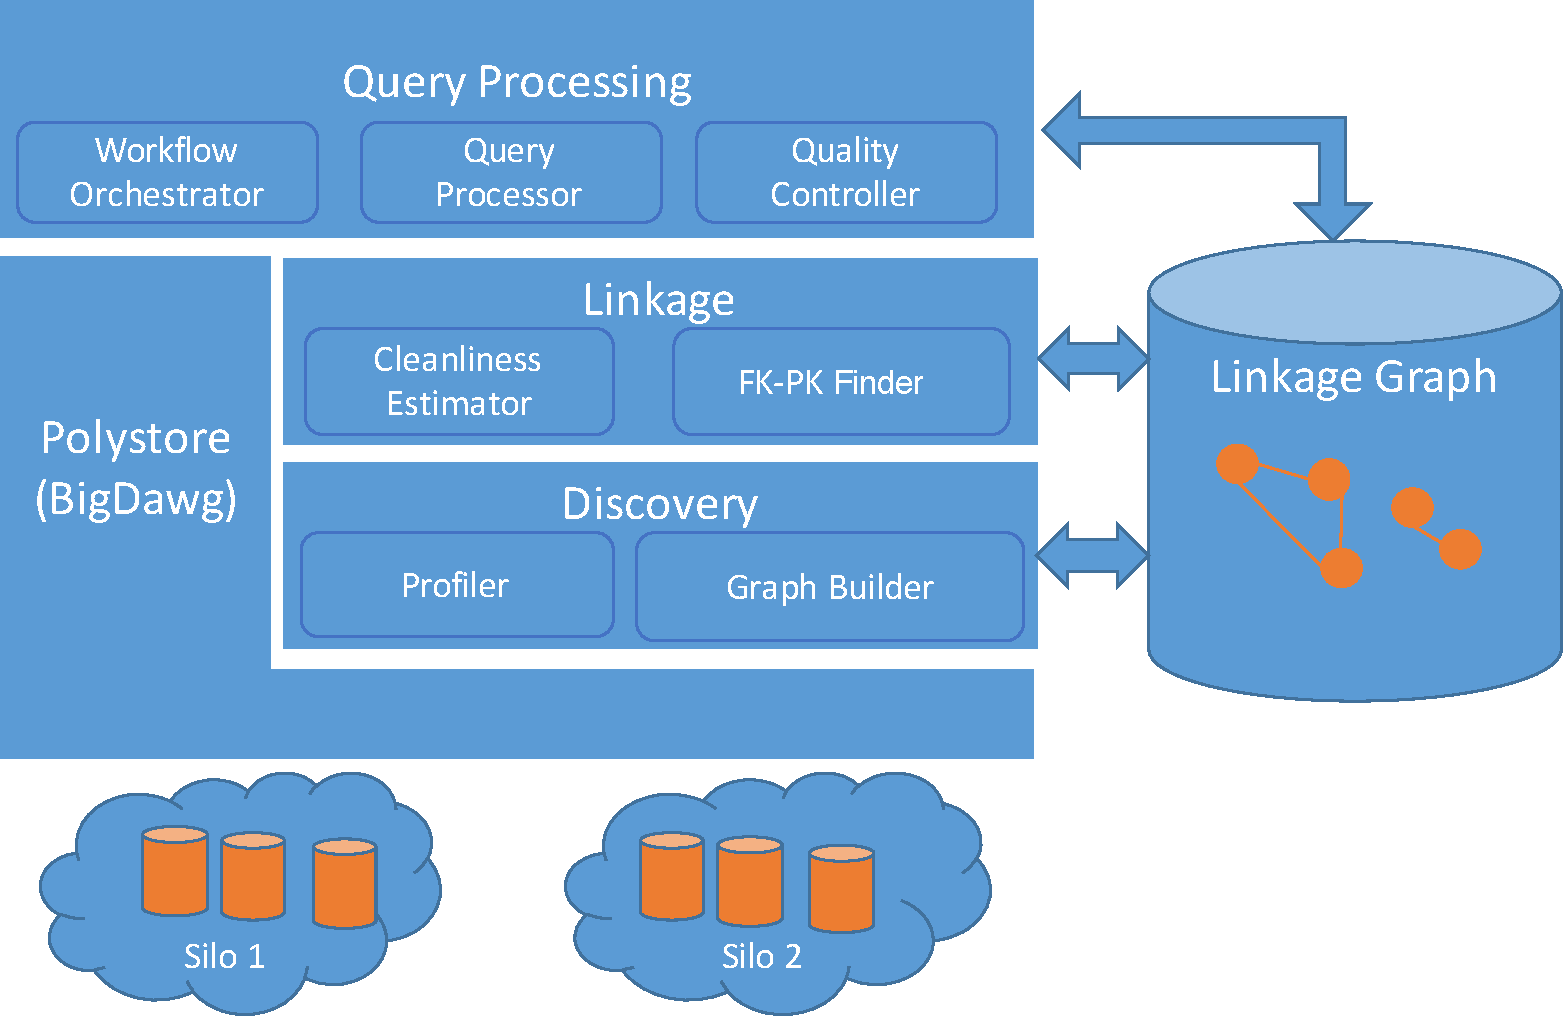
\includegraphics[width=3.5in]{arch3.pdf}
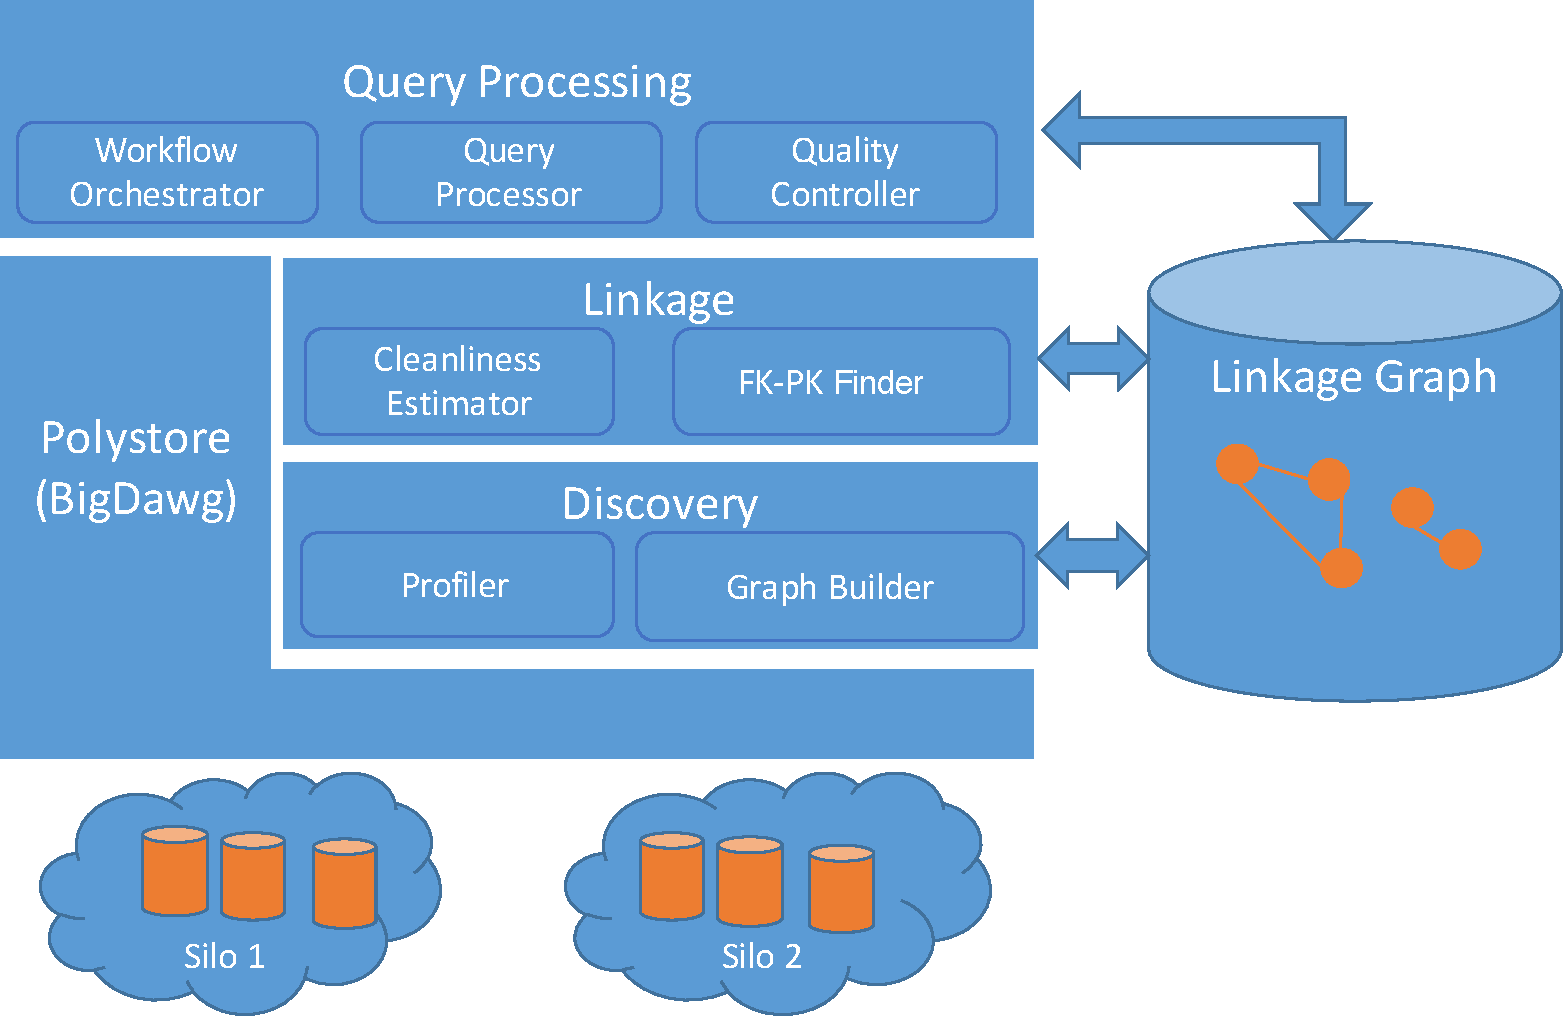
\includegraphics[width=\columnwidth]{arch3.pdf}
\caption{\dcv Architecture}
\label{fig:arch}
\end{figure}


%For example, a data scientist at Merck wants to build an drug-indication
%ontology. 
%\vspace{-.15em}
\stitle{[Linkage Graph Computation.]} The linkages amongst attributes and tables
are needed so that the user can discover interesting data, assemble relational
schemas, and run \textsf{SQL} queries on the discovered data sets. 
%All the
%linkages that can be found in linear time are built in advance during offline
%stage.  
%\srm{Graph building does not need to be done all at once:  as data
%changes and new tables are added, they can be scanned and added to the graph
%incrementally.} 
%\mourad{We could say: 
Initially, all the linkages that can be found in linear time are built during the offline stage. As existing data changes and new tables are added, the graph is incrementally updated to reflect these changes. All the other linkages, such as primary key-foreign key (\pkfk) relationships, will be
built in the background or on-demand during the online stage. Our current
prototype identifies \pkfk relationships, using inclusion dependencies. As such,
the process of building the linkage graph can be run dynamically and on-demand;
we discuss its details in Section~\ref{sec:stitching}.



%\vspace{-.15em}
\stitle{[Discovery.]} A data scientist at Merck has a hypothesis, for example,
{\it the drug Ritalin causes brain cancer in rats weighing more than 300 grams}.
His first job is to identify relevant data sets, both inside and outside of
Merck, that might contribute to testing this hypothesis. Inside the company
alone, Merck has approximately 4,000 Oracle databases and countless other
repositories. The discovery component in \dcv will assist the scientist in
finding tables of interest from all the Merck tables. Discovery queries are run
as a part of the online workflow which is discussed in
Section~\ref{sec:discovery}.

% Although discovery queries are run as a part of the online workflow, they are
% supported by profiles and indexes that are built during the offline
% processing.  Building these profiles requires looking at both the schema and
% values of every table. Consequently, we employ linear algorithms to make this
% pre-computation tractable. This module, together with the corresponding data
% structures, is discussed in Section~\ref{sec:discovery}.




%\vspace{-.15em}
\stitle{[Polystore Query Processing and Curation.]} Since organizations such as
Merck have a variety of massive-scale data storage systems, it is not feasible
to move all data to a central data warehouse. Also, it is neither economically
nor technically practical to perform data processing on all of the thousands of
databases in advance.  \dcv is built using a polystore
architecture~\cite{DBLP:journals/sigmod/DugganESBHKMMMZ15} that federates query
processing across disparate systems inside an enterprise. Our plan is to
leverage the \texttt{BigDAWG} polystore
system~\cite{DBLP:journals/pvldb/ElmoreDSBCGHHKK15} to pull data from multiple
underlying storage engines to compute the final result (or the {\em view}) that
satisfies the user's specifications.
%\vspace{-.15em}
%\stitle{[Curation Polystore]} 

%In fact, we are building on the \texttt{BigDAWG} polystore system~\cite{DBLP:journals/pvldb/ElmoreDSBCGHHKK15}. The polystore architecture can pull data out of multiple underlying storage engines as needed. 

Obviously, data cleaning, data transformation and entity consolidation must be
integrated with querying the polystore and constructing the desired user view.
This is an expensive process with the human effort required to validate cleaning
decisions being the most important cost.  Since there may be multiple views that
``solve'' a data scientist's query, each with different accuracy and human
validation cost, \dcv must estimate the cost of curating the possible views,
%to reason about the feasibility of using each one,
given a scientist's time budget.  The above aspects will be discussed in
Section~\ref{sec:curating}.


%Obviously, we want to run stitching in the background in advance to deliver the best possible response time. As noted in Section~\ref{sec:stitching}, our current prototype leverages PK-FK relationships (inclusion dependencies).
%We also plan to explore other possible relationships in the futu%The merger of polystores and data curation steps is discussed in Section~\ref{sec:curating}.re such as ???.
%Effectively, the result of stitching is a ``view'' of multiple data sources that contains the composite data of interest to the scientist.

%\vspace{-.15em}
%\stitle{[Cleanliness Estimation]} 
%Indeed, \dcv is an iterative process, the human effort will be involved in various modules. The expensive process in constructing the view mentioned above is the human effort required to validate cleaning decisions. Since there may be multiple views that ``solve'' a data scientist's query, each with different accuracy and human validation cost, \dcv must estimate the cost of curating the possible views,
%%to reason about the feasibility of using each one,
%given a scientist's time budget. 

%Estimating the cleanliness of a view entails constructing a model for the dirtiness of the data in each source data set, which we discuss in Section~\ref{sec:curating}. Also discussed in Section~\ref{sec:curating} is where in a query plan we should allocate a cleaning budget.

%\vspace{-.15em}
%\stitle{[Optimizing Stitching]} It is highly inefficient and wasteful to  discard expensive-to-construct materialized views after their initial use by a data scientist.  Hence, we assume that they are generally retained for future use.  Moreover, future materialized views  may be based off previously constructed ones or on original data sources.  As a result, there may be several ways to construct a new view, with different  costs and accuracy. Therefore, the data stitching problem must be revisited to deal with this materialization cost/accuracy trade-off.  This is the subject of Sections~\ref{sec:enhancedstitching}.\mourad{Why not merge this section with Data Stitching?}
%\vspace{-.15em}
\stitle{[Updates.]}  If a source data set is updated, these updates must be
incrementally propagated through the data curation pipeline to update downstream
materialized views.  In some cases, the human effort involved may be daunting
and the materialized view should be discarded rather than updated.  In addition,
if a scientist updates a view, we need to propagate changes to other derived
views, as well as back upstream to data sources, if this is possible.
Section~\ref{sec:updates} discusses these  issues.


%\vspace{-.15em}
\stitle{[Workflow.]} \dcv offers a workflow engine whereby data scientists can
iterate over its components in whatever order they wish. Moreover, they
need to be able to undo previous workflow steps and perform alternate branching
from the result of a workflow step.  Section~\ref{sec:workflow} discusses our
workflow management ideas.

\smallskip

We describe the state of the current implementation of \dcv in
Section~\ref{sec:wild}. We also report on initial user experience for two use
cases: the MIT data warehouse and Merck. We conclude with final remarks in Section~\ref{sec:conclusion}.

\smallskip
%\stitle{Our contributions.}
The main contribution of \dcv is that it is an ``end-to-end'' system. In
contrast, there has been much work on ``point solutions'' that solve small
pieces of the overall problem. For example, Data Wrangler~\cite{2011-wrangler}
and DataXFormer~\cite{DBLP:conf/icde/AbedjanMIOPS16} automate some aspects of
cleaning and transforming data, Data
Tamer~\cite{DBLP:conf/cidr/StonebrakerBIBCZPX13} mainly performs schema mappings
and record linkage, and DeepDive~\cite{DBLP:journals/pvldb/ShinWWSZR15} extracts
facts and structured information from large corpora of text, images and other
unstructured sources. However, no solution performs  discovery, linkage graph
computation, and polystore operations in concert. 
In addition, we have recently
studied several representative data cleaning systems on a collection of real
world data sets``from the wild''~\cite{DBLP:journals/pvldb/AbedjanCDFIOPST16}
and we found out that there was no cleaning Esperanto. 
Hence multiple tools are
required to achieve reasonable accuracy and point solutions neither offer enough functionalities nor achieve acceptable performance. Therefore an ensemble approach is needed.

